\documentclass[12pt]{article}

\usepackage[german]{babel}
\usepackage{amsmath}
\usepackage{amssymb} % to display symbols for real numbers, integers etc. Usage: \mathbb{R}
\usepackage{graphicx}
\usepackage{listings} % to display programming code
%\usepackage[ngerman]{babel}
\usepackage{color}
\usepackage{relsize} % to display scaled math symbols (big summation symbol etc.)
\usepackage{textcomp}

\DeclareGraphicsExtensions{.pdf,.jpeg,.png}
\definecolor{listinggray}{gray}{0.9}
\definecolor{lbcolor}{rgb}{0.9,0.9,0.9}
\lstset{ % to display programming code in nice colors
	backgroundcolor=\color{lbcolor},
	tabsize=4,
	rulecolor=,
	language=matlab,
		basicstyle=\scriptsize, %for extra small font size
        upquote=true,
        aboveskip={1.5\baselineskip},
        columns=fixed,
        showstringspaces=false,
        extendedchars=true,
        breaklines=true,
        prebreak = \raisebox{0ex}[0ex][0ex]{\ensuremath{\hookleftarrow}},
		frame=single, %draw frame
        showtabs=false,
        showspaces=false,
        showstringspaces=false,
        identifierstyle=\ttfamily,
        keywordstyle=\color[rgb]{0,0,1},
        commentstyle=\color[rgb]{0.133,0.545,0.133},
        stringstyle=\color[rgb]{0.627,0.126,0.941},
        numbers=left,
        stepnumber=1,
        firstnumber=1,
        numberfirstline=true,
        linewidth=14cm,
}

\title{\"Ubungsblatt 9\\ \glqq Mustererkennung\grqq}
\author{J. Cavojska, N. Lehmann, R. Toudic}
\date{06.07.2015}
\begin{document}
\maketitle
%\renewcommand{\contentsname}{Table of Contents}
\tableofcontents
\newpage

\section{Aufgabe 1 - XOR-Netzwerk mit Backpropagation trainieren}

\begin{lstlisting}[language=Matlab]
W1_init    = rand(3,2);                     % random weights 3x2 from input to layer 1
W2_init    = rand(3,1);                     % random weights 3x1 from layer 1 to layer 2
LTD        = [1 1 0; 1 0 1; 0 1 1; 0 0 0];  % labeled training data
L          = [0; 1; 1; 0];                  % labels
ATD        = [1 1 1; 1 0 1; 0 1 1; 0 0 1];  % augmented data without labels
E1         = [];                            % error history for plot
e1         = 1;                             % just for e != 0

% set initial values
W1         = W1_init;
W2         = W2_init;
alpha      = 0.1;                          % learning rate
eq1        = 0.0001;                        % error quality

% learning
for runs=1:100000
    random             = randi(4);
    L0                 = ATD(random,:);
    label              = L(random,:);
        
    % forward pass
    % layer 1
    t                  = L0 * W1;
    perceptron1_layer1 = 1.0 / (1.0 + exp(-t(:,1)));
    perceptron2_layer1 = 1.0 / (1.0 + exp(-t(:,2)));
    out_layer1         = [perceptron1_layer1, perceptron2_layer1];
    
    % layer 2
    t                  = [perceptron1_layer1, perceptron2_layer1, 1]*W2;
    perceptron1_layer2 = 1.0 / (1.0 + exp(-t));
    out_layer2         = perceptron1_layer2;
    
    % error calculation
    e1                 = perceptron1_layer2 - label;
    E1                 = horzcat(E1,e1);
    
    % backward pass
    t1                 = L0 * W1;
    s11                = (1.0 / (1+exp(-t1(:,1))))*(1-(1 / (1+exp(-t1(:,1)))));
    s12                = (1.0 / (1+exp(-t1(:,2))))*(1-(1 / (1+exp(-t1(:,2)))));
    D1                 = [s11, 0; 0, s12];
    
    t2                 = [out_layer1, 1] * W2;
    s2                 = (1 / (1+exp(-t2)))*(1-(1 / (1+exp(-t2))));
    D2                 = s2;
    
    W2_                = W2(1:2,:);
    dW1                = -alpha*D1*W2_*D2*e1'*L0;
    dW2                = -alpha*D2*e1'*[out_layer1, 1];
    W1                 = W1 + dW1';
    W2                 = W2 + dW2';

end

needed_iterations = length(E1);

% plot
figure('NumberTitle','off','Name','Aufgabe 1');
plot(E1, '.')
title('Fehlerkurven');
xlabel('Iterationen');
ylabel('Fehlerwert');
axis([-0.1 needed_iterations -1.5 1.5]);
legend('Fehlerwerte');

% gelernte Gewichte:
W1
%      6.2294    4.2282
%      6.2397    4.2218
%     -2.7229   -6.4831

W2
%      8.6958
%     -9.4197
%     -3.9711
\end{lstlisting}
Wir haben alle errors $e1$ aufgesammmelt und in einem Scatter-Plot dargestellt:\\
\begin{center}
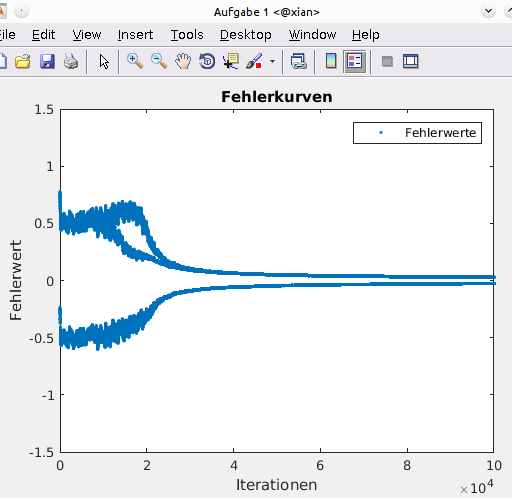
\includegraphics[width=10cm]{Bilder/errorplot_aufg1.png}
\end{center}
\newpage

\section{Aufgabe 2 - Handschriftbuchstaben klassifizieren}

Datenaufbereitung fuer Aufg. 2\\
\begin{lstlisting}[language=Matlab]
LTD        = horzcat(cTraining,labelsTraining);  % labeled training data
ATD        = horzcat(cTraining,ones(7494,1));    % augmented data without labels

LTDtest    = horzcat(cTesting,labelsTesting);  % labeled test data
ATDtest    = horzcat(cTesting,ones(3498,1));   % augmented data without labels
predictedClassk2 = [];
predictedClassk4 = [];
predictedClassk8 = [];
predictedClassk10 = [];
\end{lstlisting}

\subsection{k = 2}
Der Code fuer eine hidden layer size von 2:\\
\begin{lstlisting}[language=Matlab]
% k = 2, Training
E2         = [];           % error history for plot
e2         = 1;            % just for e != 0

% set initial values
W1         = rand(17,2);   % random weights 17x2 from layer 0 to layer 1
W2         = rand(3,10);   % random weights 3x10 from layer 1 to layer 2
alpha      = 0.01;         % learning rate
eq2        = 0.0001;       % error quality


for runs = 1:length(ATD)
    
    L0                = ATD(runs,:);
    label             = labelsTraining(runs);
        
    % forward pass
    % layer 1
    t                   = L0 * W1;
    perceptron01_layer1 = 1 / (1 + exp(-t(:,1)));
    perceptron02_layer1 = 1 / (1 + exp(-t(:,2)));
    
    out_layer1         = [perceptron01_layer1,perceptron02_layer1];
    
    % layer 2
    t                  = [out_layer1, 1]*W2;
    perceptron01_layer2 = 1 / (1 + exp(-t(1)));
    perceptron02_layer2 = 1 / (1 + exp(-t(2)));
    perceptron03_layer2 = 1 / (1 + exp(-t(3)));
    perceptron04_layer2 = 1 / (1 + exp(-t(4)));
    perceptron05_layer2 = 1 / (1 + exp(-t(5)));
    perceptron06_layer2 = 1 / (1 + exp(-t(6)));
    perceptron07_layer2 = 1 / (1 + exp(-t(7)));
    perceptron08_layer2 = 1 / (1 + exp(-t(8)));
    perceptron09_layer2 = 1 / (1 + exp(-t(9)));
    perceptron10_layer2 = 1 / (1 + exp(-t(10)));
    
    out_layer2         = [perceptron01_layer2,perceptron02_layer2,perceptron03_layer2,perceptron04_layer2,perceptron05_layer2,perceptron06_layer2,perceptron07_layer2,perceptron08_layer2,perceptron09_layer2,perceptron10_layer2];
    
    % error calculation
    labelVector = zeros(1,10);
    for labelIndex = 1:10
        if label == labelIndex
            labelVector(:,labelIndex) = 1;
        end
    end


    e2                 = out_layer2 - labelVector;
    E2                 = horzcat(E2,sum(e2));
    
    
    % backward pass
    t1                 = L0 * W1;
    s11                = (1 / (1+exp(-t1(:,1))))*(1-(1 / (1+exp(-t1(:,1)))));
    s12                = (1 / (1+exp(-t1(:,2))))*(1-(1 / (1+exp(-t1(:,2)))));
       
    D1                 = [s11,0;
                          0,s12];
    
    t2                 = [out_layer1, 1] * W2;
    s201               = (1 / (1+exp(-t2(1))))*(1-(1 / (1+exp(-t2(1)))));
    s202               = (1 / (1+exp(-t2(2))))*(1-(1 / (1+exp(-t2(2)))));
    s203               = (1 / (1+exp(-t2(3))))*(1-(1 / (1+exp(-t2(3)))));
    s204               = (1 / (1+exp(-t2(4))))*(1-(1 / (1+exp(-t2(4)))));
    s205               = (1 / (1+exp(-t2(5))))*(1-(1 / (1+exp(-t2(5)))));
    s206               = (1 / (1+exp(-t2(6))))*(1-(1 / (1+exp(-t2(6)))));
    s207               = (1 / (1+exp(-t2(7))))*(1-(1 / (1+exp(-t2(7)))));
    s208               = (1 / (1+exp(-t2(8))))*(1-(1 / (1+exp(-t2(8)))));
    s209               = (1 / (1+exp(-t2(9))))*(1-(1 / (1+exp(-t2(9)))));
    s210               = (1 / (1+exp(-t2(10))))*(1-(1 / (1+exp(-t2(10)))));
    
    D2                 = [s201,0,0,0,0,0,0,0,0,0;
                          0,s202,0,0,0,0,0,0,0,0;
                          0,0,s203,0,0,0,0,0,0,0;
                          0,0,0,s204,0,0,0,0,0,0;
                          0,0,0,0,s205,0,0,0,0,0;
                          0,0,0,0,0,s206,0,0,0,0;
                          0,0,0,0,0,0,s207,0,0,0;
                          0,0,0,0,0,0,0,s208,0,0;
                          0,0,0,0,0,0,0,0,s209,0;
                          0,0,0,0,0,0,0,0,0,s210];
    
    W2_                = W2(1:2,:);
    dW1                = -alpha*D1*W2_*D2*e2'*L0;
    dW2                = -alpha*D2*e2'*[out_layer1, 1];
    W1                 = W1 + dW1';
    W2                 = W2 + dW2';

end

needed_iterations = length(E2);

% plot
figure('NumberTitle','off','Name','Aufgabe 2, k=2');
plot(E2, '.')
title('Fehlerkurven');
xlabel('Iterationen');
ylabel('Fehlerwert');
axis([-0.1 needed_iterations -10 10]);
legend('Fehlerwerte');


% k = 2, Testing

correctly_predicted = 0;
for runs = 1:length(ATDtest)
    
    L0                = ATDtest(runs,:);
    label             = labelsTesting(runs);
        
    % forward pass
    % layer 1
    t                   = L0 * W1;
    perceptron01_layer1 = 1 / (1 + exp(-t(:,1)));
    perceptron02_layer1 = 1 / (1 + exp(-t(:,2)));
    
    out_layer1         = [perceptron01_layer1,perceptron02_layer1];
    
    % layer 2
    t                  = [out_layer1, 1]*W2;
    perceptron01_layer2 = 1 / (1 + exp(-t(1)));
    perceptron02_layer2 = 1 / (1 + exp(-t(2)));
    perceptron03_layer2 = 1 / (1 + exp(-t(3)));
    perceptron04_layer2 = 1 / (1 + exp(-t(4)));
    perceptron05_layer2 = 1 / (1 + exp(-t(5)));
    perceptron06_layer2 = 1 / (1 + exp(-t(6)));
    perceptron07_layer2 = 1 / (1 + exp(-t(7)));
    perceptron08_layer2 = 1 / (1 + exp(-t(8)));
    perceptron09_layer2 = 1 / (1 + exp(-t(9)));
    perceptron10_layer2 = 1 / (1 + exp(-t(10)));
    
    out_layer2         = [perceptron01_layer2,perceptron02_layer2,perceptron03_layer2,perceptron04_layer2,perceptron05_layer2,perceptron06_layer2,perceptron07_layer2,perceptron08_layer2,perceptron09_layer2,perceptron10_layer2];
    
    % prediction calculation
    prediction = 999;  % initial value
    predictionVal = max(out_layer2);
    for index = 1:length(out_layer2)
        if out_layer2(1, index) == predictionVal
            prediction = index - 1;
        end
    end
    predictedClassk2 = vertcat(predictedClassk2, prediction);
    if prediction == label
        correctly_predicted = correctly_predicted + 1;
    end
end


confusionMatrix_k2 = confusionmat(labelsTesting, predictedClassk2)

%confusionMatrix_k2 =
%
%     0     0     0     0     0     0   363     0     0     0
%     0     0     0     0     0     0   364     0     0     0
%     0     0     0     0     0     0   364     0     0     0
%     0     0     0     0     0     0   336     0     0     0
%     0     0     0     0     0     0   364     0     0     0
%     0     0     0     0     0     0   335     0     0     0
%     0     0     0     0     0     0   336     0     0     0
%     0     0     0     0     0     0   364     0     0     0
%     0     0     0     0     0     0   336     0     0     0
%     0     0     0     0     0     0   336     0     0     0

klass_guete = correctly_predicted / size(ATDtest, 1)

%klass_guete =
%
%    0.0961

\end{lstlisting}
Ein Plot des beim Training mit $k = 2$ entstandenen Errors:\\
\begin{center}
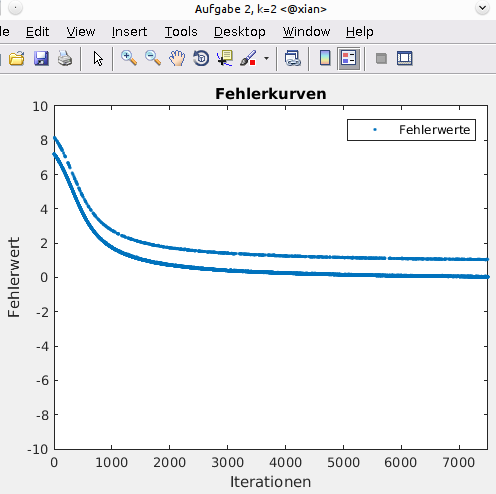
\includegraphics[width=10cm]{Bilder/errorplot_aufg2_k2.png}
\end{center}

\subsection{k = 4}
\begin{lstlisting}[language=Matlab]
% k = 4, Training
E4         = [];           % error history for plot
e4         = 1;            % just for e != 0

% set initial values
W1         = rand(17,4);   % random weights 17x2 from layer 0 to layer 1
W2         = rand(5,10);   % random weights 5x10 from layer 1 to layer 2
alpha      = 0.01;         % learning rate

for runs = 1:length(ATD)
    
    L0                = ATD(runs,:);
    label             = labelsTraining(runs);
        
    % forward pass
    % layer 1
    t                   = L0 * W1;
    perceptron01_layer1 = 1 / (1 + exp(-t(:,1)));
    perceptron02_layer1 = 1 / (1 + exp(-t(:,2)));
    perceptron03_layer1 = 1 / (1 + exp(-t(:,3)));
    perceptron04_layer1 = 1 / (1 + exp(-t(:,4)));
    
    out_layer1         = [perceptron01_layer1,perceptron02_layer1,perceptron03_layer1,perceptron04_layer1];
    
    % layer 2
    t                  = [out_layer1, 1]*W2;
    perceptron01_layer2 = 1 / (1 + exp(-t(1)));
    perceptron02_layer2 = 1 / (1 + exp(-t(2)));
    perceptron03_layer2 = 1 / (1 + exp(-t(3)));
    perceptron04_layer2 = 1 / (1 + exp(-t(4)));
    perceptron05_layer2 = 1 / (1 + exp(-t(5)));
    perceptron06_layer2 = 1 / (1 + exp(-t(6)));
    perceptron07_layer2 = 1 / (1 + exp(-t(7)));
    perceptron08_layer2 = 1 / (1 + exp(-t(8)));
    perceptron09_layer2 = 1 / (1 + exp(-t(9)));
    perceptron10_layer2 = 1 / (1 + exp(-t(10)));
    
    out_layer2         = [perceptron01_layer2,perceptron02_layer2,perceptron03_layer2,perceptron04_layer2,perceptron05_layer2,perceptron06_layer2,perceptron07_layer2,perceptron08_layer2,perceptron09_layer2,perceptron10_layer2];
    
    % error calculation
    labelVector = zeros(1,10);
    for labelIndex = 1:10
        if label == labelIndex
            labelVector(:,labelIndex) = 1;
        end
    end
    e4                 = out_layer2 - labelVector;
    E4                 = horzcat(E4,sum(e4));
    
    
    % backward pass
    t1                 = L0 * W1;
    s11                = (1 / (1+exp(-t1(:,1))))*(1-(1 / (1+exp(-t1(:,1)))));
    s12                = (1 / (1+exp(-t1(:,2))))*(1-(1 / (1+exp(-t1(:,2)))));
    s13                = (1 / (1+exp(-t1(:,3))))*(1-(1 / (1+exp(-t1(:,3)))));
    s14                = (1 / (1+exp(-t1(:,4))))*(1-(1 / (1+exp(-t1(:,4)))));
       
    D1                 = [s11,0,0,0;
                          0,s12,0,0;
                          0,0,s13,0;
                          0,0,0,s14];
    
    t2                 = [out_layer1, 1] * W2;
    s201               = (1 / (1+exp(-t2(1))))*(1-(1 / (1+exp(-t2(1)))));
    s202               = (1 / (1+exp(-t2(2))))*(1-(1 / (1+exp(-t2(2)))));
    s203               = (1 / (1+exp(-t2(3))))*(1-(1 / (1+exp(-t2(3)))));
    s204               = (1 / (1+exp(-t2(4))))*(1-(1 / (1+exp(-t2(4)))));
    s205               = (1 / (1+exp(-t2(5))))*(1-(1 / (1+exp(-t2(5)))));
    s206               = (1 / (1+exp(-t2(6))))*(1-(1 / (1+exp(-t2(6)))));
    s207               = (1 / (1+exp(-t2(7))))*(1-(1 / (1+exp(-t2(7)))));
    s208               = (1 / (1+exp(-t2(8))))*(1-(1 / (1+exp(-t2(8)))));
    s209               = (1 / (1+exp(-t2(9))))*(1-(1 / (1+exp(-t2(9)))));
    s210               = (1 / (1+exp(-t2(10))))*(1-(1 / (1+exp(-t2(10)))));
    
    D2                 = [s201,0,0,0,0,0,0,0,0,0;
                          0,s202,0,0,0,0,0,0,0,0;
                          0,0,s203,0,0,0,0,0,0,0;
                          0,0,0,s204,0,0,0,0,0,0;
                          0,0,0,0,s205,0,0,0,0,0;
                          0,0,0,0,0,s206,0,0,0,0;
                          0,0,0,0,0,0,s207,0,0,0;
                          0,0,0,0,0,0,0,s208,0,0;
                          0,0,0,0,0,0,0,0,s209,0;
                          0,0,0,0,0,0,0,0,0,s210];
    
    W2_                = W2(1:4,:);
    dW1                = -alpha*D1*W2_*D2*e4'*L0;
    dW2                = -alpha*D2*e4'*[out_layer1, 1];
    W1                 = W1 + dW1';
    W2                 = W2 + dW2';

end

needed_iterations = length(E4);

% plot
figure('NumberTitle','off','Name','Aufgabe 2, k=4');
plot(E4, '.')
title('Fehlerkurven');
xlabel('Iterationen');
ylabel('Fehlerwert');
axis([-0.1 needed_iterations -10 10]);
legend('Fehlerwerte');


% k = 4, Testing

correctly_predicted = 0;
for runs = 1:length(ATDtest)
    
    L0                = ATDtest(runs,:);
    label             = labelsTesting(runs);
        
    % forward pass
    % layer 1
    t                   = L0 * W1;
    perceptron01_layer1 = 1 / (1 + exp(-t(:,1)));
    perceptron02_layer1 = 1 / (1 + exp(-t(:,2)));
    perceptron03_layer1 = 1 / (1 + exp(-t(:,3)));
    perceptron04_layer1 = 1 / (1 + exp(-t(:,4)));
    
    out_layer1         = [perceptron01_layer1,perceptron02_layer1,perceptron03_layer1,perceptron04_layer1];
    
    % layer 2
    t                  = [out_layer1, 1]*W2;
    perceptron01_layer2 = 1 / (1 + exp(-t(1)));
    perceptron02_layer2 = 1 / (1 + exp(-t(2)));
    perceptron03_layer2 = 1 / (1 + exp(-t(3)));
    perceptron04_layer2 = 1 / (1 + exp(-t(4)));
    perceptron05_layer2 = 1 / (1 + exp(-t(5)));
    perceptron06_layer2 = 1 / (1 + exp(-t(6)));
    perceptron07_layer2 = 1 / (1 + exp(-t(7)));
    perceptron08_layer2 = 1 / (1 + exp(-t(8)));
    perceptron09_layer2 = 1 / (1 + exp(-t(9)));
    perceptron10_layer2 = 1 / (1 + exp(-t(10)));
    
    out_layer2         = [perceptron01_layer2,perceptron02_layer2,perceptron03_layer2,perceptron04_layer2,perceptron05_layer2,perceptron06_layer2,perceptron07_layer2,perceptron08_layer2,perceptron09_layer2,perceptron10_layer2];
    
    % prediction calculation
    prediction = 999;  % initial value
    predictionVal = max(out_layer2);
    for index = 1:length(out_layer2)
        if out_layer2(1, index) == predictionVal
            prediction = index - 1;
        end
    end
    predictedClassk4 = vertcat(predictedClassk4, prediction);
    if prediction == label
        correctly_predicted = correctly_predicted + 1;
    end
end


confusionMatrix_k4 = confusionmat(labelsTesting, predictedClassk4)

%confusionMatrix_k4 =
%
%     0     0     0     0     0     0   363     0     0     0
%     0     0     0     0     0     0   364     0     0     0
%     0     0     0     0     0     0   364     0     0     0
%     0     0     0     0     0     0   336     0     0     0
%     0     0     0     0     0     0   364     0     0     0
%     0     0     0     0     0     0   335     0     0     0
%     0     0     0     0     0     0   336     0     0     0
%     0     0     0     0     0     0   364     0     0     0
%     0     0     0     0     0     0   336     0     0     0
%     0     0     0     0     0     0   336     0     0     0

klass_guete = correctly_predicted / size(ATDtest, 1)

%klass_guete =
%
%    0.0961
\end{lstlisting}
Ein Plot des beim Training mit $k = 4$ entstandenen Errors:\\
\begin{center}
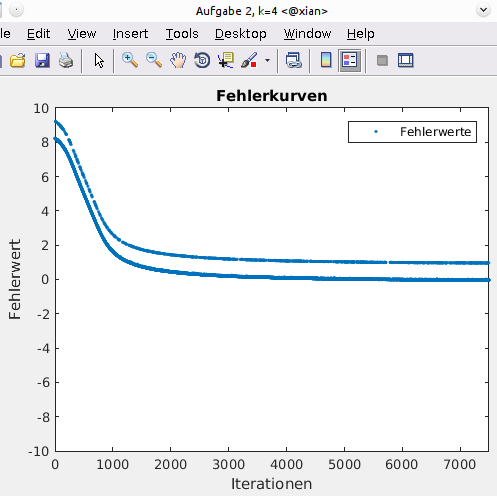
\includegraphics[width=10cm]{Bilder/errorplot_aufg2_k4.png}
\end{center}

\subsection{k = 8}
\begin{lstlisting}[language=Matlab]
% k = 8, Training
E8         = [];           % error history for plot
e8         = 1;            % just for e != 0

% set initial values
W1         = rand(17,8);   % random weights 17x2 from layer 0 to layer 1
W2         = rand(9,10);   % random weights 3x10 from layer 1 to layer 2
alpha      = 0.01;         % learning rate

for runs = 1:length(ATD)
    
    L0     = ATD(runs,:);
    label  = labelsTraining(runs);
        
    % forward pass
    % layer 1
    t                   = L0 * W1;
    perceptron01_layer1 = 1 / (1 + exp(-t(:,1)));
    perceptron02_layer1 = 1 / (1 + exp(-t(:,2)));
    perceptron03_layer1 = 1 / (1 + exp(-t(:,3)));
    perceptron04_layer1 = 1 / (1 + exp(-t(:,4)));
    perceptron05_layer1 = 1 / (1 + exp(-t(:,5)));
    perceptron06_layer1 = 1 / (1 + exp(-t(:,6)));
    perceptron07_layer1 = 1 / (1 + exp(-t(:,7)));
    perceptron08_layer1 = 1 / (1 + exp(-t(:,8)));
    
    out_layer1         = [perceptron01_layer1,perceptron02_layer1,perceptron03_layer1,perceptron04_layer1,perceptron05_layer1,perceptron06_layer1,perceptron07_layer1,perceptron08_layer1];
    
    % layer 2
    t                  = [out_layer1, 1]*W2;
    perceptron01_layer2 = 1 / (1 + exp(-t(1)));
    perceptron02_layer2 = 1 / (1 + exp(-t(2)));
    perceptron03_layer2 = 1 / (1 + exp(-t(3)));
    perceptron04_layer2 = 1 / (1 + exp(-t(4)));
    perceptron05_layer2 = 1 / (1 + exp(-t(5)));
    perceptron06_layer2 = 1 / (1 + exp(-t(6)));
    perceptron07_layer2 = 1 / (1 + exp(-t(7)));
    perceptron08_layer2 = 1 / (1 + exp(-t(8)));
    perceptron09_layer2 = 1 / (1 + exp(-t(9)));
    perceptron10_layer2 = 1 / (1 + exp(-t(10)));
    
    out_layer2         = [perceptron01_layer2,perceptron02_layer2,perceptron03_layer2,perceptron04_layer2,perceptron05_layer2,perceptron06_layer2,perceptron07_layer2,perceptron08_layer2,perceptron09_layer2,perceptron10_layer2];
    
    % error calculation
    labelVector = zeros(1,10);
    for labelIndex = 1:10
        if label == labelIndex
            labelVector(:,labelIndex) = 1;
        end
    end

    e8                 = out_layer2 - labelVector;
    E8                 = horzcat(E8,sum(e8));    
    
    % backward pass
    t1                 = L0 * W1;
    s11                = (1 / (1+exp(-t1(:,1))))*(1-(1 / (1+exp(-t1(:,1)))));
    s12                = (1 / (1+exp(-t1(:,2))))*(1-(1 / (1+exp(-t1(:,2)))));
    s13                = (1 / (1+exp(-t1(:,3))))*(1-(1 / (1+exp(-t1(:,3)))));
    s14                = (1 / (1+exp(-t1(:,4))))*(1-(1 / (1+exp(-t1(:,4)))));
    s15                = (1 / (1+exp(-t1(:,5))))*(1-(1 / (1+exp(-t1(:,5)))));
    s16                = (1 / (1+exp(-t1(:,6))))*(1-(1 / (1+exp(-t1(:,6)))));
    s17                = (1 / (1+exp(-t1(:,7))))*(1-(1 / (1+exp(-t1(:,7)))));
    s18                = (1 / (1+exp(-t1(:,8))))*(1-(1 / (1+exp(-t1(:,8)))));
       
    D1                 = [s11,0,0,0,0,0,0,0;
                          0,s12,0,0,0,0,0,0;
                          0,0,s13,0,0,0,0,0;
                          0,0,0,s14,0,0,0,0;
                          0,0,0,0,s15,0,0,0;
                          0,0,0,0,0,s16,0,0;
                          0,0,0,0,0,0,s17,0;
                          0,0,0,0,0,0,0,s18];
    
    t2                 = [out_layer1, 1] * W2;
    s201               = (1 / (1+exp(-t2(1))))*(1-(1 / (1+exp(-t2(1)))));
    s202               = (1 / (1+exp(-t2(2))))*(1-(1 / (1+exp(-t2(2)))));
    s203               = (1 / (1+exp(-t2(3))))*(1-(1 / (1+exp(-t2(3)))));
    s204               = (1 / (1+exp(-t2(4))))*(1-(1 / (1+exp(-t2(4)))));
    s205               = (1 / (1+exp(-t2(5))))*(1-(1 / (1+exp(-t2(5)))));
    s206               = (1 / (1+exp(-t2(6))))*(1-(1 / (1+exp(-t2(6)))));
    s207               = (1 / (1+exp(-t2(7))))*(1-(1 / (1+exp(-t2(7)))));
    s208               = (1 / (1+exp(-t2(8))))*(1-(1 / (1+exp(-t2(8)))));
    s209               = (1 / (1+exp(-t2(9))))*(1-(1 / (1+exp(-t2(9)))));
    s210               = (1 / (1+exp(-t2(10))))*(1-(1 / (1+exp(-t2(10)))));
    
    D2                 = [s201,0,0,0,0,0,0,0,0,0;
                          0,s202,0,0,0,0,0,0,0,0;
                          0,0,s203,0,0,0,0,0,0,0;
                          0,0,0,s204,0,0,0,0,0,0;
                          0,0,0,0,s205,0,0,0,0,0;
                          0,0,0,0,0,s206,0,0,0,0;
                          0,0,0,0,0,0,s207,0,0,0;
                          0,0,0,0,0,0,0,s208,0,0;
                          0,0,0,0,0,0,0,0,s209,0;
                          0,0,0,0,0,0,0,0,0,s210];
    
    W2_                = W2(1:8,:);
    dW1                = -alpha*D1*W2_*D2*e8'*L0;
    dW2                = -alpha*D2*e8'*[out_layer1, 1];
    W1                 = W1 + dW1';
    W2                 = W2 + dW2';

end

needed_iterations = length(E8);

% plot
figure('NumberTitle','off','Name','Aufgabe 2, k=8');
plot(E8, '.')
title('Fehlerkurven');
xlabel('Iterationen');
ylabel('Fehlerwert');
axis([-0.1 needed_iterations -10 10]);
legend('Fehlerwerte');


% k = 8, Testing

correctly_predicted = 0;
for runs = 1:length(ATDtest)
    
    L0     = ATDtest(runs,:);
    label  = labelsTesting(runs);
        
    % forward pass
    % layer 1
    t                   = L0 * W1;
    perceptron01_layer1 = 1 / (1 + exp(-t(:,1)));
    perceptron02_layer1 = 1 / (1 + exp(-t(:,2)));
    perceptron03_layer1 = 1 / (1 + exp(-t(:,3)));
    perceptron04_layer1 = 1 / (1 + exp(-t(:,4)));
    perceptron05_layer1 = 1 / (1 + exp(-t(:,5)));
    perceptron06_layer1 = 1 / (1 + exp(-t(:,6)));
    perceptron07_layer1 = 1 / (1 + exp(-t(:,7)));
    perceptron08_layer1 = 1 / (1 + exp(-t(:,8)));
    
    out_layer1         = [perceptron01_layer1,perceptron02_layer1,perceptron03_layer1,perceptron04_layer1,perceptron05_layer1,perceptron06_layer1,perceptron07_layer1,perceptron08_layer1];
    
    % layer 2
    t                  = [out_layer1, 1]*W2;
    perceptron01_layer2 = 1 / (1 + exp(-t(1)));
    perceptron02_layer2 = 1 / (1 + exp(-t(2)));
    perceptron03_layer2 = 1 / (1 + exp(-t(3)));
    perceptron04_layer2 = 1 / (1 + exp(-t(4)));
    perceptron05_layer2 = 1 / (1 + exp(-t(5)));
    perceptron06_layer2 = 1 / (1 + exp(-t(6)));
    perceptron07_layer2 = 1 / (1 + exp(-t(7)));
    perceptron08_layer2 = 1 / (1 + exp(-t(8)));
    perceptron09_layer2 = 1 / (1 + exp(-t(9)));
    perceptron10_layer2 = 1 / (1 + exp(-t(10)));
    
    out_layer2         = [perceptron01_layer2,perceptron02_layer2,perceptron03_layer2,perceptron04_layer2,perceptron05_layer2,perceptron06_layer2,perceptron07_layer2,perceptron08_layer2,perceptron09_layer2,perceptron10_layer2];
    
    % prediction calculation
    prediction = 999;  % initial value
    predictionVal = max(out_layer2);
    for index = 1:length(out_layer2)
        if out_layer2(1, index) == predictionVal
            prediction = index - 1;
        end
    end
    predictedClassk8 = vertcat(predictedClassk8, prediction);
    if prediction == label
        correctly_predicted = correctly_predicted + 1;
    end

end


confusionMatrix_k8 = confusionmat(labelsTesting, predictedClassk8)

%confusionMatrix_k8 =
%
%     0     0     0     0     0     0   363     0     0     0
%     0     0     0     0     0     0   364     0     0     0
%     0     0     0     0     0     0   364     0     0     0
%     0     0     0     0     0     0   336     0     0     0
%     0     0     0     0     0     0   364     0     0     0
%     0     0     0     0     0     0   335     0     0     0
%     0     0     0     0     0     0   336     0     0     0
%     0     0     0     0     0     0   364     0     0     0
%     0     0     0     0     0     0   336     0     0     0
%     0     0     0     0     0     0   336     0     0     0


klass_guete = correctly_predicted / size(ATDtest, 1)

%klass_guete =
%
%    0.0961
\end{lstlisting}
Ein Plot des beim Training mit $k = 8$ entstandenen Errors:\\
\begin{center}
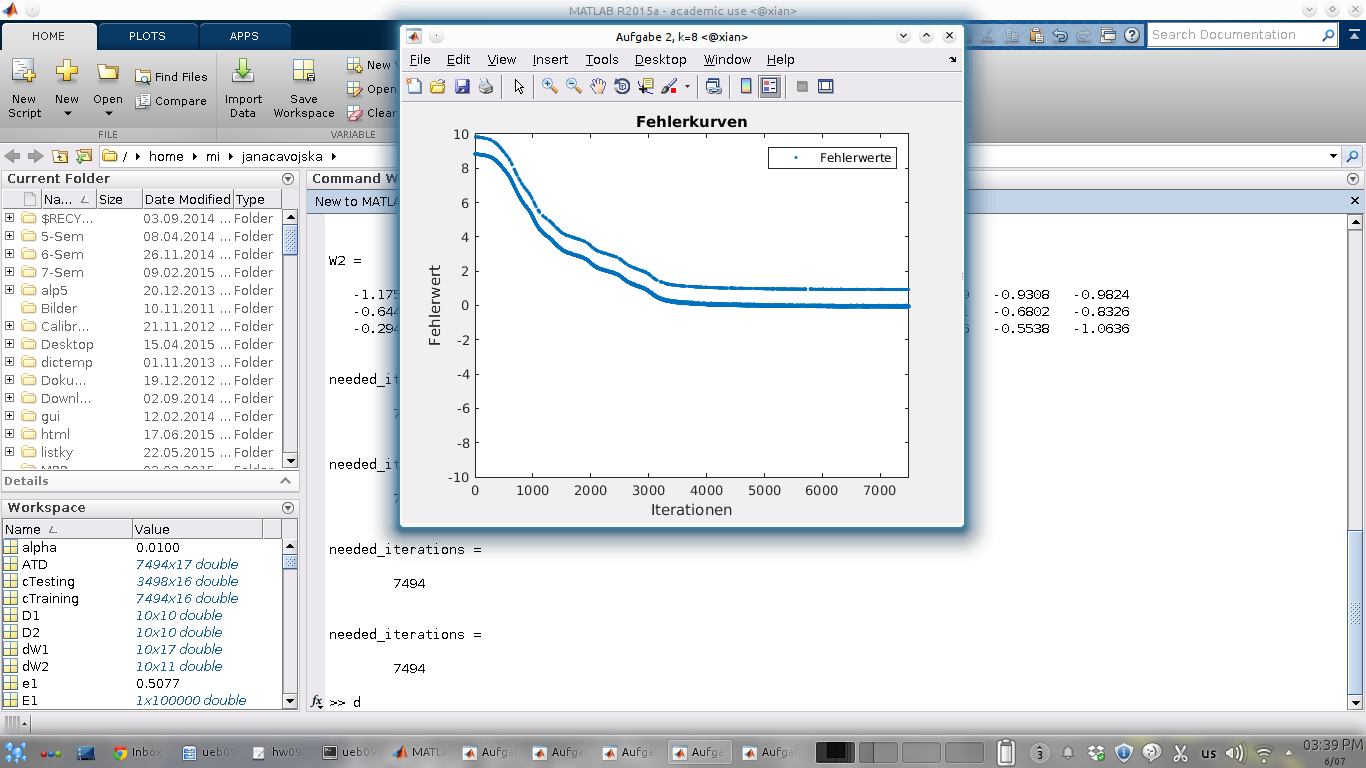
\includegraphics[width=10cm]{Bilder/errorplot_aufg2_k8.png}
\end{center}
\newpage

\subsection{k = 10}
\begin{lstlisting}[language=Matlab]
% k = 10, Training
E10        = [];           % error history for plot
e10        = 1;            % just for e != 0

% set initial values
W1         = rand(17,10);  % random weights 17x2 from layer 0 to layer 1
W2         = rand(11,10);  % random weights 3x10 from layer 1 to layer 2
alpha      = 0.01;         % learning rate

for runs = 1:length(ATD)
    
    L0                = ATD(runs,:);
    label             = labelsTraining(runs);
        
    % forward pass
    % layer 1
    t                   = L0 * W1;
    perceptron01_layer1 = 1 / (1 + exp(-t(:,1)));
    perceptron02_layer1 = 1 / (1 + exp(-t(:,2)));
    perceptron03_layer1 = 1 / (1 + exp(-t(:,3)));
    perceptron04_layer1 = 1 / (1 + exp(-t(:,4)));
    perceptron05_layer1 = 1 / (1 + exp(-t(:,5)));
    perceptron06_layer1 = 1 / (1 + exp(-t(:,6)));
    perceptron07_layer1 = 1 / (1 + exp(-t(:,7)));
    perceptron08_layer1 = 1 / (1 + exp(-t(:,8)));
    perceptron09_layer1 = 1 / (1 + exp(-t(:,9)));
    perceptron10_layer1 = 1 / (1 + exp(-t(:,10)));
    
    out_layer1         = [perceptron01_layer1,perceptron02_layer1,perceptron03_layer1,perceptron04_layer1,perceptron05_layer1,perceptron06_layer1,perceptron07_layer1,perceptron08_layer1,perceptron09_layer1,perceptron10_layer1];
    
    % layer 2
    t                  = [out_layer1, 1]*W2;
    perceptron01_layer2 = 1 / (1 + exp(-t(1)));
    perceptron02_layer2 = 1 / (1 + exp(-t(2)));
    perceptron03_layer2 = 1 / (1 + exp(-t(3)));
    perceptron04_layer2 = 1 / (1 + exp(-t(4)));
    perceptron05_layer2 = 1 / (1 + exp(-t(5)));
    perceptron06_layer2 = 1 / (1 + exp(-t(6)));
    perceptron07_layer2 = 1 / (1 + exp(-t(7)));
    perceptron08_layer2 = 1 / (1 + exp(-t(8)));
    perceptron09_layer2 = 1 / (1 + exp(-t(9)));
    perceptron10_layer2 = 1 / (1 + exp(-t(10)));
    
    out_layer2         = [perceptron01_layer2,perceptron02_layer2,perceptron03_layer2,perceptron04_layer2,perceptron05_layer2, perceptron06_layer2,perceptron07_layer2,perceptron08_layer2,perceptron09_layer2,perceptron10_layer2];
    
    % error calculation
    labelVector = zeros(1,10);
    for labelIndex = 1:10
        if label == labelIndex
            labelVector(:,labelIndex) = 1;
        end
    end
    e10                = out_layer2 - labelVector;
    E10                = horzcat(E10,sum(e10));
    
    % backward pass
    t1                 = L0 * W1;
    s101               = (1 / (1+exp(-t1(:,1))))*(1-(1 / (1+exp(-t1(:,1)))));
    s102               = (1 / (1+exp(-t1(:,2))))*(1-(1 / (1+exp(-t1(:,2)))));
    s103               = (1 / (1+exp(-t1(:,3))))*(1-(1 / (1+exp(-t1(:,3)))));
    s104               = (1 / (1+exp(-t1(:,4))))*(1-(1 / (1+exp(-t1(:,4)))));
    s105               = (1 / (1+exp(-t1(:,5))))*(1-(1 / (1+exp(-t1(:,5)))));
    s106               = (1 / (1+exp(-t1(:,6))))*(1-(1 / (1+exp(-t1(:,6)))));
    s107               = (1 / (1+exp(-t1(:,7))))*(1-(1 / (1+exp(-t1(:,7)))));
    s108               = (1 / (1+exp(-t1(:,8))))*(1-(1 / (1+exp(-t1(:,8)))));
    s109               = (1 / (1+exp(-t1(:,9))))*(1-(1 / (1+exp(-t1(:,9)))));
    s110               = (1 / (1+exp(-t1(:,10))))*(1-(1 / (1+exp(-t1(:,10)))));
       
    D1                 = [s101,0,0,0,0,0,0,0,0,0;
                          0,s102,0,0,0,0,0,0,0,0;
                          0,0,s103,0,0,0,0,0,0,0;
                          0,0,0,s104,0,0,0,0,0,0;
                          0,0,0,0,s105,0,0,0,0,0;
                          0,0,0,0,0,s106,0,0,0,0;
                          0,0,0,0,0,0,s107,0,0,0;
                          0,0,0,0,0,0,0,s108,0,0;
                          0,0,0,0,0,0,0,0,s109,0;
                          0,0,0,0,0,0,0,0,0,s110];
    
    t2                 = [out_layer1, 1] * W2;
    s201               = (1 / (1+exp(-t2(1))))*(1-(1 / (1+exp(-t2(1)))));
    s202               = (1 / (1+exp(-t2(2))))*(1-(1 / (1+exp(-t2(2)))));
    s203               = (1 / (1+exp(-t2(3))))*(1-(1 / (1+exp(-t2(3)))));
    s204               = (1 / (1+exp(-t2(4))))*(1-(1 / (1+exp(-t2(4)))));
    s205               = (1 / (1+exp(-t2(5))))*(1-(1 / (1+exp(-t2(5)))));
    s206               = (1 / (1+exp(-t2(6))))*(1-(1 / (1+exp(-t2(6)))));
    s207               = (1 / (1+exp(-t2(7))))*(1-(1 / (1+exp(-t2(7)))));
    s208               = (1 / (1+exp(-t2(8))))*(1-(1 / (1+exp(-t2(8)))));
    s209               = (1 / (1+exp(-t2(9))))*(1-(1 / (1+exp(-t2(9)))));
    s210               = (1 / (1+exp(-t2(10))))*(1-(1 / (1+exp(-t2(10)))));
    
    D2                 = [s201,0,0,0,0,0,0,0,0,0;
                          0,s202,0,0,0,0,0,0,0,0;
                          0,0,s203,0,0,0,0,0,0,0;
                          0,0,0,s204,0,0,0,0,0,0;
                          0,0,0,0,s205,0,0,0,0,0;
                          0,0,0,0,0,s206,0,0,0,0;
                          0,0,0,0,0,0,s207,0,0,0;
                          0,0,0,0,0,0,0,s208,0,0;
                          0,0,0,0,0,0,0,0,s209,0;
                          0,0,0,0,0,0,0,0,0,s210];
    
    W2_                = W2(1:10,:);
    dW1                = -alpha*D1*W2_*D2*e10'*L0;
    dW2                = -alpha*D2*e10'*[out_layer1, 1];
    W1                 = W1 + dW1';
    W2                 = W2 + dW2';

end

needed_iterations = length(E10);

% plot
figure('NumberTitle','off','Name','Aufgabe 2, k=10');
plot(E10, '.')
title('Fehlerkurven');
xlabel('Iterationen');
ylabel('Fehlerwert');
axis([-0.1 needed_iterations -10 10]);
legend('Fehlerwerte');


% k = 10, Testing
correctly_predicted = 0;
for runs = 1:length(ATDtest)
    
    L0                = ATDtest(runs,:);
    label             = labelsTesting(runs);
        
    % forward pass
    % layer 1
    t                   = L0 * W1;
    perceptron01_layer1 = 1 / (1 + exp(-t(:,1)));
    perceptron02_layer1 = 1 / (1 + exp(-t(:,2)));
    perceptron03_layer1 = 1 / (1 + exp(-t(:,3)));
    perceptron04_layer1 = 1 / (1 + exp(-t(:,4)));
    perceptron05_layer1 = 1 / (1 + exp(-t(:,5)));
    perceptron06_layer1 = 1 / (1 + exp(-t(:,6)));
    perceptron07_layer1 = 1 / (1 + exp(-t(:,7)));
    perceptron08_layer1 = 1 / (1 + exp(-t(:,8)));
    perceptron09_layer1 = 1 / (1 + exp(-t(:,9)));
    perceptron10_layer1 = 1 / (1 + exp(-t(:,10)));
    
    out_layer1         = [perceptron01_layer1,perceptron02_layer1,perceptron03_layer1,perceptron04_layer1,perceptron05_layer1,perceptron06_layer1,perceptron07_layer1,perceptron08_layer1,perceptron09_layer1,perceptron10_layer1];
    
    % layer 2
    t                  = [out_layer1, 1]*W2;
    perceptron01_layer2 = 1 / (1 + exp(-t(1)));
    perceptron02_layer2 = 1 / (1 + exp(-t(2)));
    perceptron03_layer2 = 1 / (1 + exp(-t(3)));
    perceptron04_layer2 = 1 / (1 + exp(-t(4)));
    perceptron05_layer2 = 1 / (1 + exp(-t(5)));
    perceptron06_layer2 = 1 / (1 + exp(-t(6)));
    perceptron07_layer2 = 1 / (1 + exp(-t(7)));
    perceptron08_layer2 = 1 / (1 + exp(-t(8)));
    perceptron09_layer2 = 1 / (1 + exp(-t(9)));
    perceptron10_layer2 = 1 / (1 + exp(-t(10)));
    
    out_layer2         = [perceptron01_layer2,perceptron02_layer2,perceptron03_layer2,perceptron04_layer2,perceptron05_layer2, perceptron06_layer2,perceptron07_layer2,perceptron08_layer2,perceptron09_layer2,perceptron10_layer2];
    
    % prediction calculation
    prediction = 999;  % initial value
    predictionVal = max(out_layer2);
    for index = 1:length(out_layer2)
        if out_layer2(1, index) == predictionVal
            prediction = index - 1;
        end
    end
    predictedClassk10 = vertcat(predictedClassk10, prediction);
    if prediction == label
        correctly_predicted = correctly_predicted + 1;
    end
end


confusionMatrix_k10 = confusionmat(labelsTesting, predictedClassk10)

%confusionMatrix_k10 =
%
%     0   363     0     0     0     0     0     0     0     0
%     0   364     0     0     0     0     0     0     0     0
%     0   364     0     0     0     0     0     0     0     0
%     0   336     0     0     0     0     0     0     0     0
%     0   364     0     0     0     0     0     0     0     0
%     0   335     0     0     0     0     0     0     0     0
%     0   336     0     0     0     0     0     0     0     0
%     0   364     0     0     0     0     0     0     0     0
%     0   336     0     0     0     0     0     0     0     0
%     0   336     0     0     0     0     0     0     0     0


klass_guete = correctly_predicted / size(ATDtest, 1)

%klass_guete =
%
%    0.1041
\end{lstlisting}
Ein Plot des beim Training mit $k = 10$ entstandenen Errors:\\
\begin{center}
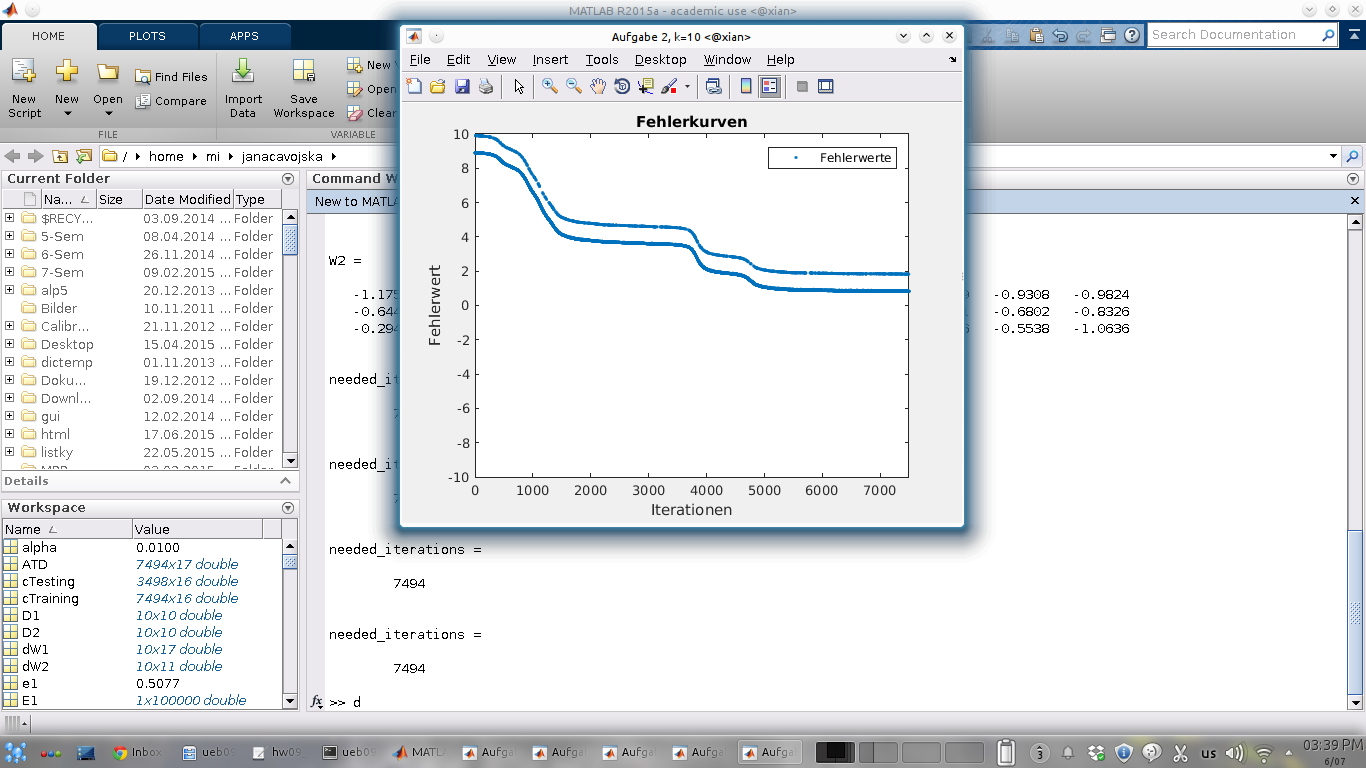
\includegraphics[width=10cm]{Bilder/errorplot_aufg2_k10.png}
\end{center}

\end{document}